\chapter{Experimental Approach}

Measurements were primarily carried out in a PWJ facility a schematic of which is shown in Figure~\ref{fg:expSet}. Air from a centrifugal fan passed through a series of screens and entered a plenum settling chamber. The air then passed through a honeycomb layer and into a two-dimensional contraction of ratio 16:1. The exit of the rectangular nozzle had a width $b =$  5 mm with an aspect ratio of 128. A strip of sand paper was installed across the facility floor, past the nozzle exit, which trips the boundary layer. This trip was used to minimize, as much as possible, the influence of the forcing on the inner wall layer transition. Most measurements were carried out at a nominal jet Reynolds number $Re_j = b V_j/ \nu \approx 5960$, where $V_j$ is nominal PWJ exit centerline velocity and $\nu$ the kinematic viscosity. A speaker produced the forcing in the plenum chamber. A range of forcing Strouhal numbers were consider spanning $St= f_fb/V_j \approx 0.28 - 5.7 \times 10^{-3}$. Here, $f_f$ was the forcing frequency. All perturbations considered were large-perturbations to the base flow as with respect to the outer scales the perturbation were such that $U_m/f_f>1.6 \delta$. 

\begin{figure}[h!]
	\centering
	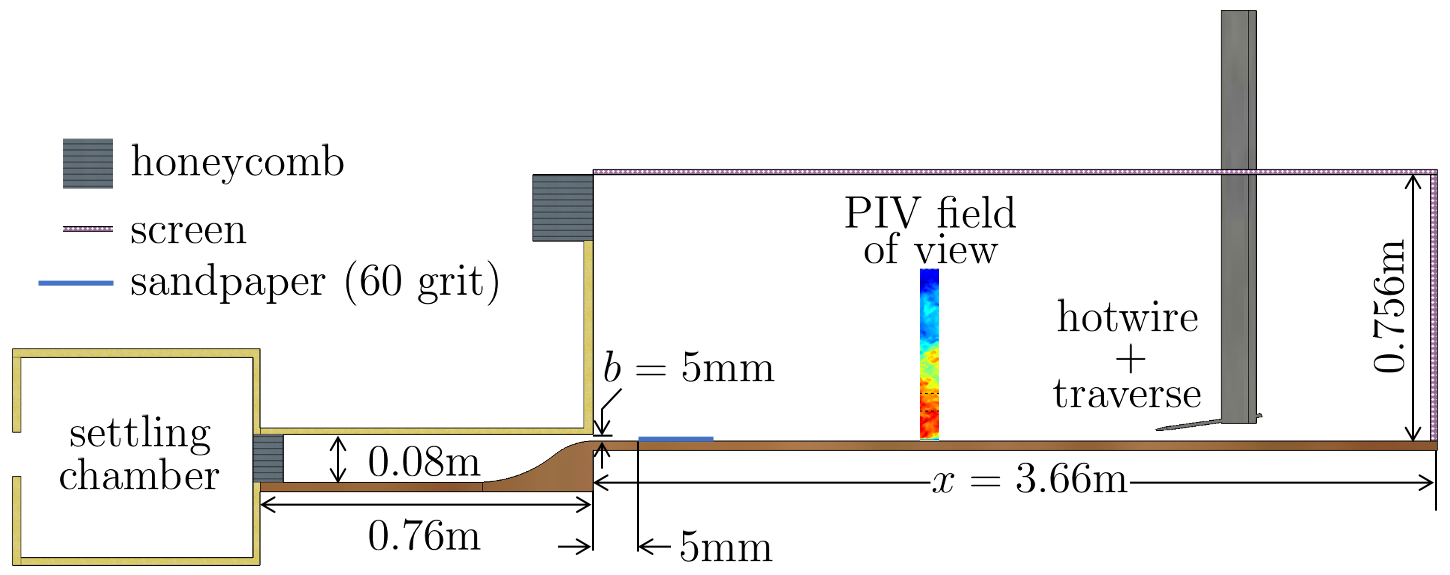
\includegraphics[width=.99\textwidth]{pics/expSch.png}
	\caption{A Schematic showing the salient features of the experimental set up.}
	\label{fg:expSet}
\end{figure}

Hot-wire anemometry (HWA) based measurements were carried out at several streamwise locations spanning $x/b = 1$ to $x/b = 162$. The hot-wire sensors were boundary-layer type probes with a diameter $d$ =2.5 \textmu m at a nominal aspect ratio of $l/d = 200$. Complementary time-resolved particle image velocimetry (PIV) measurements were also carried out. These measurements were centered at a nominal downstream location of $x/b=137$. These measurements resulted in a single wall-normal slice of temporally resolved measurements. Hence, these measurements  are comparable to an array of synchronous, multi-component hot-wire measurements. The wall-normal mean velocity $\overline{w}$ in a PWJ is non-zero therefore, HWA based measurements measure an effective velocity $U$. On the other hand PIV based measurements measures both components of the velocity i.e., the streamwise and wall-normal velocities ($u$ and $w$ respectively). The wall-normal ordinate is $z$ and the streamwise ordinate is $x$. 

The PIV based measurements were a mosaic of two cameras at different magnifications. One of the cameras focused on the inner boundary layer was at a higher magnification with a final interrogation window of $\Delta z^+ \times \Delta x^+ \approx 4 \times 4$. The top camera at a lower magnification had a final interrogation window of $\Delta z^+ \times \Delta x^+ \approx 6 \times 6$. The superscript $^+$ is indicative of normalization with respect to viscous or inner units. The friction velocity $U_\tau$ was measured using a curve fit process where the careful near wall measurements were carried out using HWA. For the rest of this report, the superscript 0 is used to identify unperturbed quantities while the superscript * is used to denote perturbed quantities.  Also, the PWJ flow is broadly separated into an inner wall region which spans wall-normal locations less than the location of the maximum velocity i.e., $z<z_m$ (see schematic of Figure~\ref{fg:pwj_sch})). The region above $z>z_m$ is the outer jet region of the PWJ.